%&xelatex
\documentclass[xcolor=svgnames]{beamer}
\usepackage[british]{babel}
\usepackage[T1]{fontenc}
\usepackage[utf8]{inputenc}

\usepackage{tcolorbox}
\usepackage{graphicx}
\usepackage{booktabs}

%\usetheme[block=fill,progressbar=frametitle]{metropolis}
\usepackage{lmodern}

\usepackage{bytefield}
\usepackage{tikz}
\usetikzlibrary{shapes.misc, shapes.symbols, positioning, calc}

\usepackage{xcolor}
\usepackage[normalem]{ulem}

\useinnertheme{default}
\useoutertheme{infolines}
\usecolortheme{seahorse}
\setbeamercolor*{alerted text}{fg=blue!75!black}
\setbeamertemplate{blocks}[rounded]
\setbeamertemplate{itemize item}[triangle]
\setbeamertemplate{itemize subitem}[circle]
\setbeamertemplate{itemize subsubitem}[square]

\usecolortheme{rose}
\definecolor{NUblue}{RGB}{62,141,165}
\definecolor{NUbluedark}{RGB}{40,119,143}
\setbeamercolor*{palette primary}{use=structure,fg=white,bg=NUblue}
\setbeamercolor*{palette quaternary}{fg=white,bg=NUbluedark}
\setbeamercolor{section in head/foot}{fg=white,bg=NUbluedark}
\setbeamercolor{subsection in head/foot}{fg=white,bg=NUblue}
\setbeamercolor{frametitle}{fg=NUbluedark!150,bg=NUblue!40}
\setbeamercolor{title in head/foot}{fg=white,bg=NUblue}
\setbeamercolor{author in head/foot}{fg=white, bg=NUbluedark}
\setbeamercolor{date in head/foot}{fg=white, bg=NUblue!60}
\setbeamercolor{title}{fg=NUbluedark!150,bg=NUblue!30}
\setbeamercolor{date}{fg=NUbluedark!150}
\setbeamercolor{block title}{fg=white,bg=NUblue}

\title{Control systems and Computer Networks}
\subtitle{Embedded and Networked Systems}

\author{Dr Alun Moon}
\date{Lecture 1.1}
\begin{document}
\frame{\maketitle}

\begin{frame}{Embedded Systems}
  \begin{itemize}[<+->]
  \item A \alert{Computer} that is built into \alert{electronic devices} to
        simplify the design or enhance performance.
  \item Often the user is unaware of the presence of the computer.
  \item Interacts with  the physical world.
  \item \alert{Networked} communicates with other devices and computers to
        co-ordinate actions and distribute the workload.
\end{itemize}
\end{frame}

\begin{frame}{Characteristics}
\begin{itemize}[<+->]
  \item Reliability
  \begin{itemize}
    \item Mission Critical
    \item life threatening
    \item 24/7/365
    \item Can't reboot
  \end{itemize}
    \item Performance
    \begin{itemize}
      \item \alert{Soft} and \alert{Hard} Real-Time requirements.
      \item External events trigger actions.
      \item Some degree of multi-tasking (interrupts/RTOS)
      \end{itemize}
    \item Cost
    \begin{itemize}
      \item Consumer market -- minimise manufacturing costs
      \item Fast time to market required
      \item No chance for future \emph{in service} modifications
    \end{itemize}
    \item Limited Interaction
    \begin{itemize}
      \item difficult to debug
      \item demanding technical and programming work
    \end{itemize}
    \item \colorbox{NUblue!40}{Challenging, demanding, fun, \& very satisfying to work on}
\end{itemize}
\end{frame}

\begin{frame}{Jacqard Loom}{Early industrial automation}
\begin{columns}[onlytextwidth]
\begin{column}{.6\textwidth}
    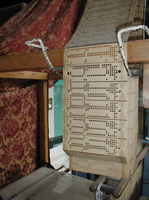
\includegraphics{Jacquard-loom-cards.png}
\end{column}
\begin{column}{.4\textwidth}
    \begin{itemize}
        \item Punched Cards controlling loom
        \item 1804
        \item manufacturing textiles with such complex patterns as brocade, damask and matelassé
    \end{itemize}
\end{column}
\end{columns}
\end{frame}

\begin{frame}{Ubiquitous }
    \begin{itemize}[<+->]
        \item Embedded systems outnumber PC "Computers"
        \begin{itemize}
            \item $\approx 100 : 1$
        \end{itemize}
        \item Many unseen
        \begin{itemize}
            \item 5 or more in the kitchen
            \item at least 2 on the outside of the PC
            \item several in this room
        \end{itemize}
        \item A "Computer" is a collection of several micro-cotrollers/processors
    \end{itemize}

    \begin{block}{examples}<+->
      \begin{itemize}
        \item More than 86 billion ARM®-based chips shipped to date.
        \item Microchip -- PIC and AVR (ATmega in Arduino)
      \end{itemize}
    \end{block}
\end{frame}

\begin{frame}{Following in the Steps and Leaps}{Apollo Guidance Computer}
\begin{itemize}[<+->]
  \item First use of integrated circuits to build a computer.
  \begin{itemize}
    \item Kick started IC industry
    \item NASA/MIT/Apollo consumed 60\% of the IC production in the USA
  \end{itemize}
  \item Early use of concurrency via extensive use of interrupts.
  \item One of the first significant avionics control systems
  \item High reliability.  (MTBF 50000 hours)
  \item Pioneered many embedded, safety-critical techniques.
  \begin{itemize}
    \item Margaret Hamilton, of the Massachusetts Institute of Technology,
      with her colleagues, she developed the building blocks for modern
      ``software engineering,''
      a term Hamilton coined.
    \item Apollo 11, 1201 and 1202 alarms
  \end{itemize}
  \item May be the first ``networked'' embedded system

\end{itemize}
\end{frame}

\begin{frame}{Modern Network of systems}
    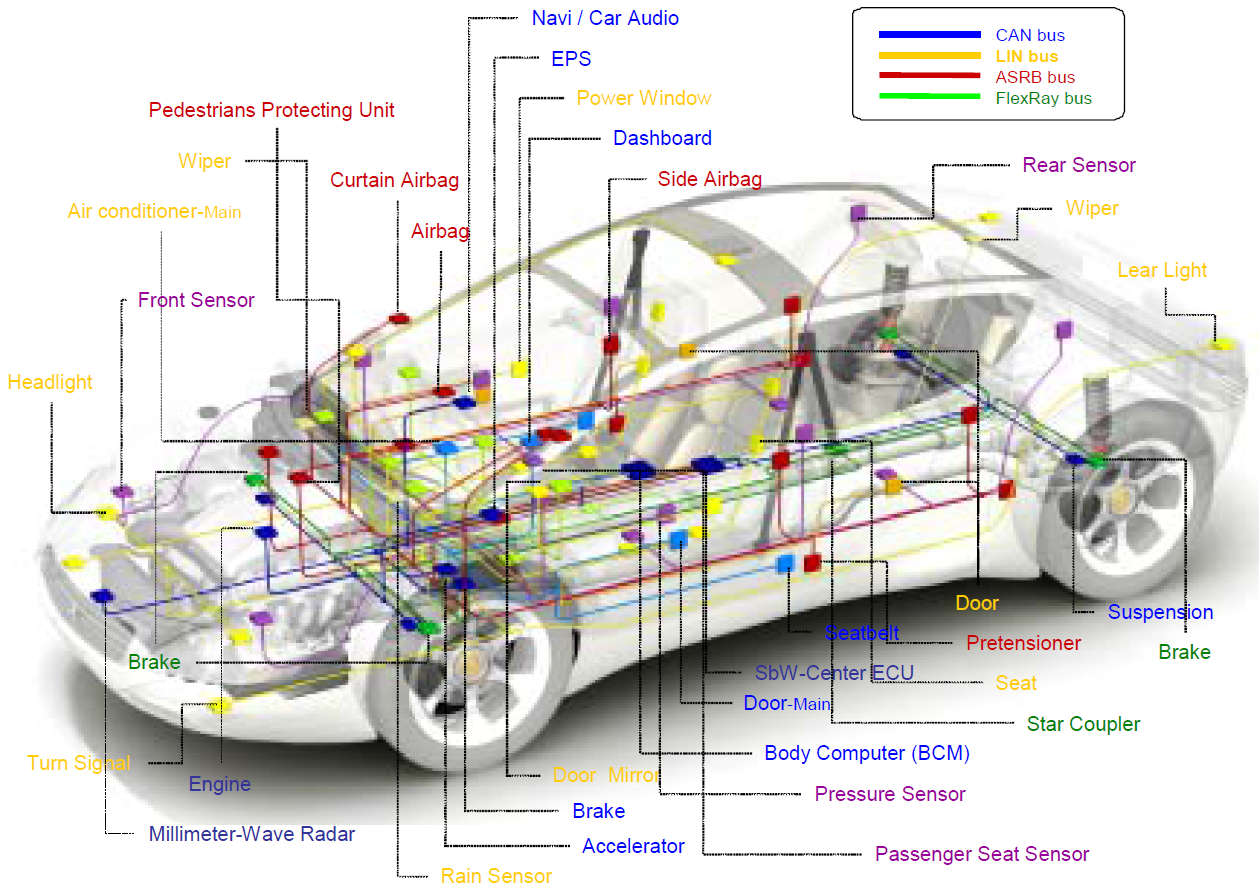
\includegraphics[width=\textwidth]{CAN-car.png}
\end{frame}

\newcommand\redout{\bgroup\markoverwith
{\textcolor{red}{\rule[0.3ex]{2pt}{2pt}}}\ULon}
\begin{frame}{Control}
    \begin{itemize}[<+->]
        \item Deal with physical signals
        \item Physical Quantities
        \item Sense environment
        \begin{itemize}
          \item Voltages
          \item Temperatures
          \item Button Presses
        \end{itemize}
        \item Effect environment
        \begin{itemize}
            \item Lights \& Heating
            \item Motors -- motion
            \item Change physical quantities
        \end{itemize}
        \item \only<+(-1)>{Virtual Reality}\only<+(-1)->{\redout{Virtual} Reality}
    \end{itemize}
\end{frame}

\begin{frame}{We Deal with Reality}
    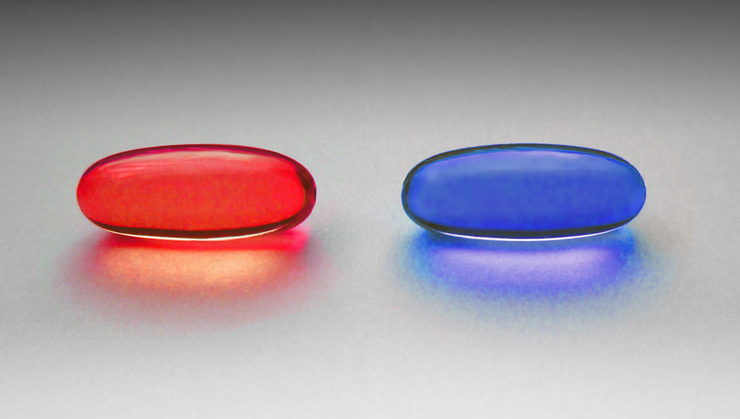
\includegraphics{Red_and_blue_pill.png}\\
    \pause
    \begin{quote}
        You take the red pill -- you stay in Wonderland, and I show you how deep the rabbit hole goes.\\
        ~\hspace*{\fill}{\textit Morpheus, The Matrix}
    \end{quote}
    \begin{tikzpicture}[remember picture, overlay]
        \node[forbidden sign, draw, scale=8, very thick, xshift=1.7mm, yshift=0.8mm, line width=3mm] at (current page.center) {} ;
    \end{tikzpicture}
\end{frame}


\end{document}
%%%%======================
